% Chapter Template

\chapter{Execution Management} % Main chapter title

\label{chapter:plan_execution} % Change X to a consecutive number; for referencing this chapter elsewhere, use \ref{ChapterX}

\lhead{Chapter 5. \emph{Execution Management}} % Change X to a consecutive number; this is for the header on each page - perhaps a shortened title

This chapter shows the Execution Management layer of our system. Section \ref{sec:plan_execution-intro} introduces the subject. Section \ref{sec:plan_execution-overview} shows an overview of this layer, with its characteristics and components. Section \ref{sec:plan_execution-action_executor} shows the main aspects of the Action Execution module, while \ref{sec:plan_execution-collaborative_planners} shows the framework we use to execute human-robot joint actions.


\section{Introduction}
\label{sec:plan_execution-intro}
Acting in a human-crowded environment is a difficult problem. Even when acting independently, the robot needs to ensure human safety, by taking others into account when planning and stopping if its actions could bring harm; to perform legible movements, so that its actions can be understand by humans (studied, for example, in \cite{dragan2013legibility}); and to be robust, trying to complete its task even in front of unexpect conditions. 

These issues show us that humans should not be treated as simple obstacles by the robot, but need specialized reasoning and execution algorithms.

When performing a cooperative action with the human the robot needs to continuously monitor its partner, checking if he is involved in the task, stopping to wait for him, adapting its movements, and eventually abandoning the task. For example, if the robot is giving an object to a human, it will have to choose a position for its arm where the human can easily reach the object, change this position if the human is moving, and abandon the task if the human leaves the area.

\cite{bussy2012proactive} studied how to execute a transportation scenario jointly with a human partner, but the work is based more on haptic and control issues than actual reasoning, an area of the problem not deeply investigated.

\section{Overview}
\label{sec:plan_execution-overview}

We built an execution layer with different characteristics:
\begin{itemize}
\item Flexibility. The system is built in order to be easily expandable, adding new actions, without having an impact on the rest of the architecture.
\item Human-Awareness. The system is able to take humans into account during planning, considering aspects such as the visibility of the robot, the legibility of its motions, and the confort of the human. Human-Awareness is maintained during the execution of motions, stopping the robot if its movements could endanger a human.
\item Support for joint actions . The system supports joint actions, by specifically representing them in a special framework.
\end{itemize}

These ideas are represented in the following modules, as shown in figure~\ref{fig:plan_execution:architecture}.
\begin{itemize}
	\item Action Executor. This module executes the robot's actions in a robust, human-aware, and flexible way.
	\item Collaborative Planners. This set of planners are used to execute human-robot joint actions, allowing the robot to adapt its actions to the collaborators.
	\item Motion Planners and Executors. These planners are in charge of choosing trajectories for the robot, taking into account the environment and the present agents. We will not discuss this component, as it is outside the boundaries of this work. More details can be found in \cite{Sisbot2008,Mainprice2011,Pandey2010}.
\end{itemize}


\begin{figure}[h!]
	\centering
	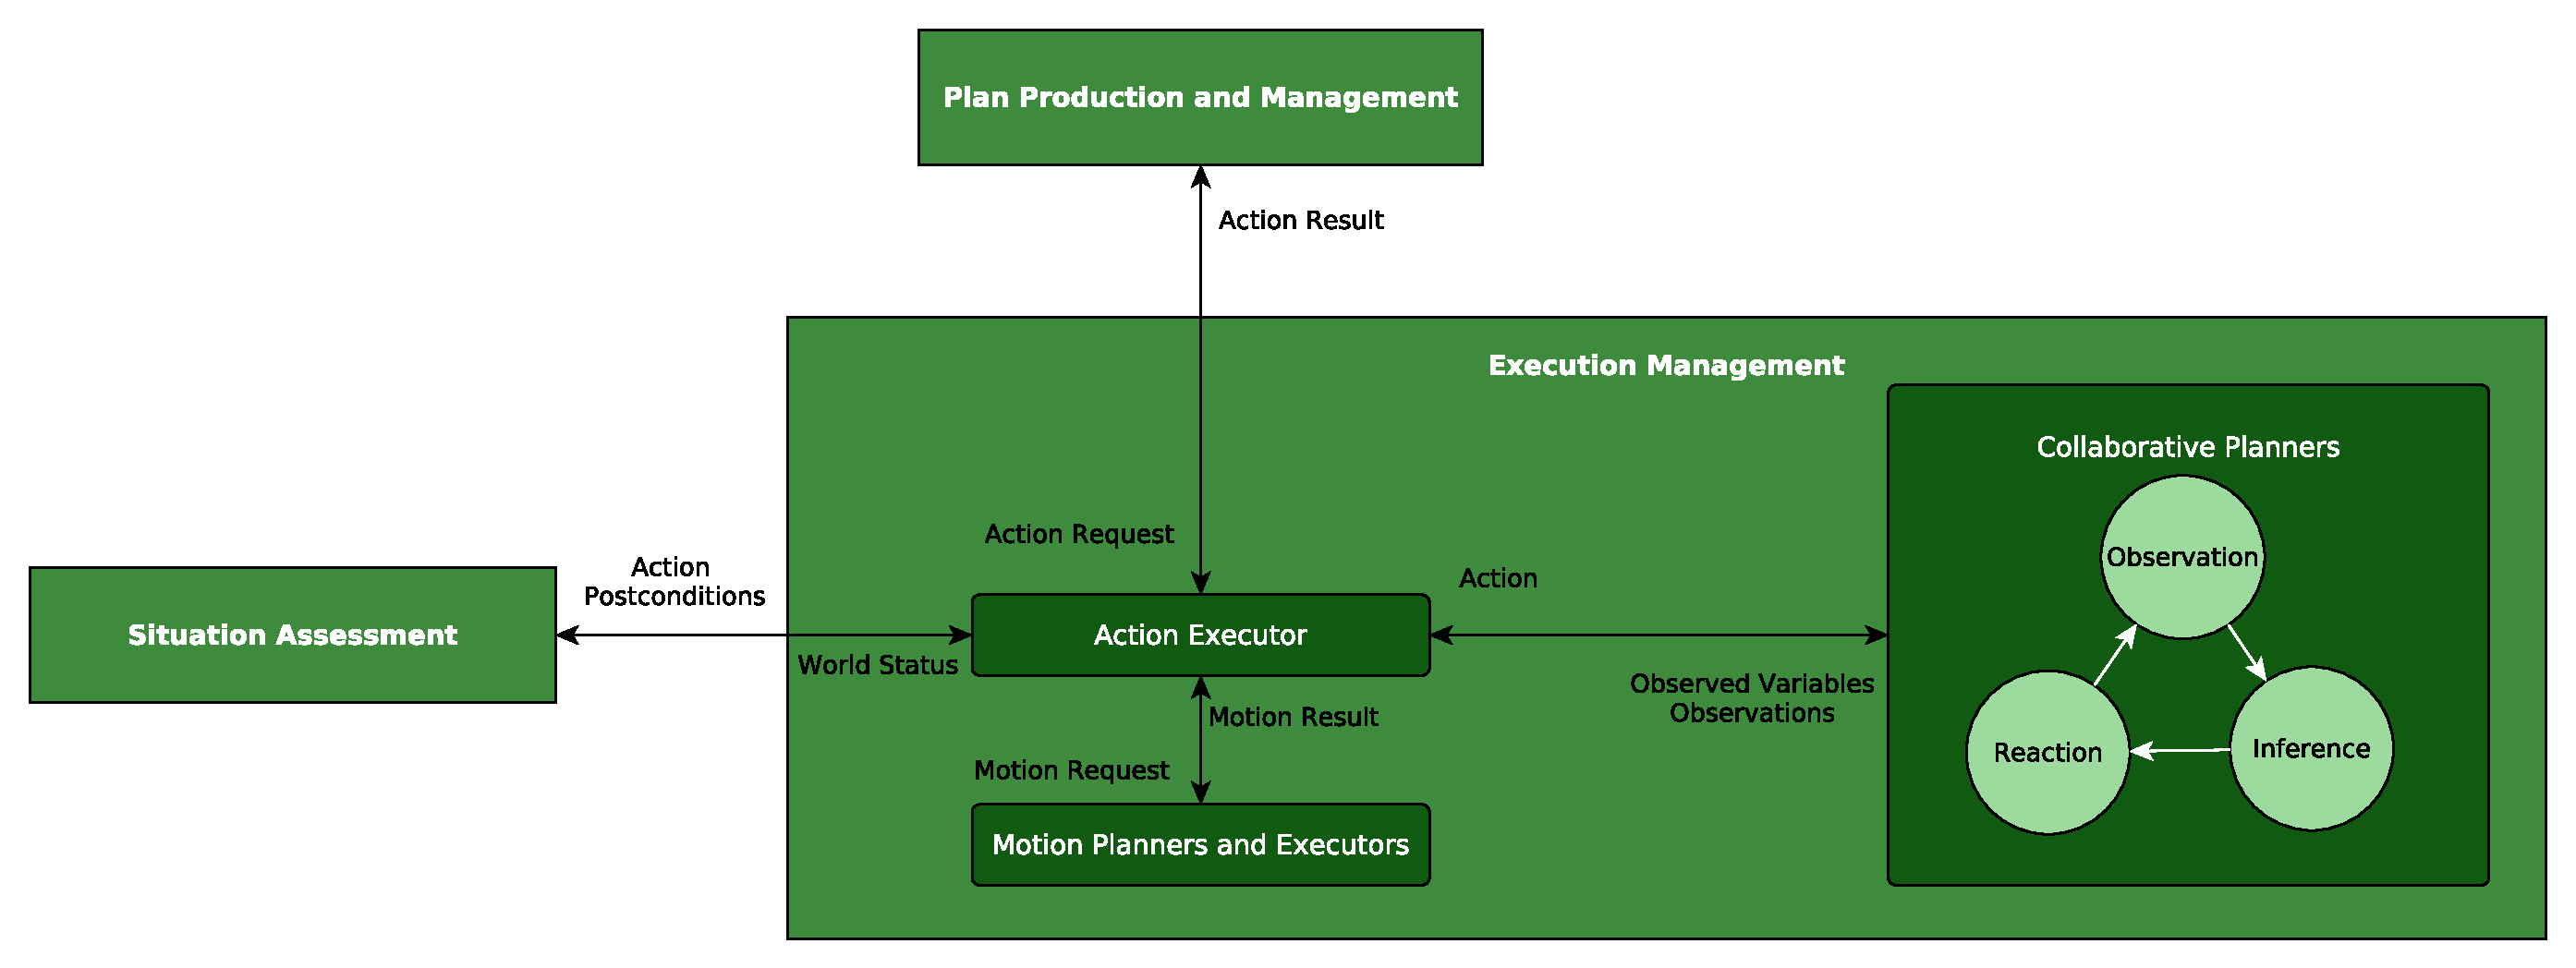
\includegraphics[clip,scale=0.38]{img/plan_execution/architecture.pdf}
	\caption[The architecture of the Execution Management layer]{The architecture of the Execution Management layer. Dark green rectangles represent modules, while light green rectangles layers. Arrows represent message exchanged between components, with the label detailing the message. The white ellipses represens, and their arrows, represent the process of the Collaborative Planners, explained in Section \ref{sec:plan_execution-collaborative_planners} }
	\label{fig:plan_execution:architecture}
\end{figure}


Parts of this chapter where presented in~\cite{fioreiser2014}.

\section{Action Executor}
\label{sec:plan_execution-action_executor}
The action executor handles action requests from the Plan Production and Management layer. Each action, as explained in subsection~\ref{sec:situation_assessment-belief_management}, is a tuple $(name, preconditions, target, postconditions)$. The execution of an action is handled in several steps:
\begin{itemize}
\item Check Preconditions. The system can check if the preconditions of the actions are valid by sending a query to the Situation Assessment layer. If the preconditions are not valid, the module returns the \textit{action\_not\_executable} error.
\item Execute Action. The action is executed, by communicating with the Motion Planners and Executors and, if the current action is a joint action, with the Collaborative Planners.
\item Set Postconditions. The postconditions of the action are set in the Situation Assessment layer.
\end{itemize}

The execution of an action can fail, and in that case the world status is updated consequently. For example, if the robot was trying to pick an object, and the action fails, the object will be considered as \textit{not reachable} by the robot in the current world status. When the Plan Management and Production replans, the system could look for a plan where the robot changes position and tries again the pick, or even asks another agent to give him the object.

Actions can be paused and resumed, for example because a human steps in the trajectory planned by the robot. The robot is also able to show some social clues during an action, for example by moving its head toward the action's $target$. 

\section{Collaborative Planners} 
\label{sec:plan_execution-collaborative_planners}
When executing joint actions with humans, the robot needs to continuously observe its partner and react appropriately. The robot's action should be based on different aspects. First of all, the robot should act differently depending on the current status and level of advancement of the task. Second, the robot should consider the status of the world, in order to take appropriate actions. Then, as we said, the robot should observe its partner's behavior, which can give different information. Of course, the robot should coordinate with the human's movements. For example, if the two agents are performing an handover, and the human extends his hand, the robot should extend its arm to bring the object in a reachable position.

Observing the human's action can give us more subtle information, that represent how much he is engaged in the task. For example, in the case of the handover, if the human is oriented toward the robot and extending his hand, we can assume that the human is currently engaged and cooperating. If, instead, the human is looking in another direction, or moving away, we can infer that he is currently doing something else, and perhaps has even abandoned the task.

To reason on all these variables and produce an appropriate reaction, we introduced a special framework to manage cooperative actions, called the Collaborative Planners, based on hierarchical Mixed Observability Markov Decision Processes (MOMDP). Using an MMODP we can model both observed variables, like the task and world status, and hidden variables, like the engagement level of the human, which we can measure from observations. Using a hierarchy of models, as explained in \cite{pineau2001hierarchical}, we can represent complex scenarios and tasks with smaller, simpler models, that can be solved more easily, and expand them by adding more actions and complex behaviors as we see fit.

When the system is executing a joint action between the robot and a human, the Action Executor will contact the related Collaborative Planner.  The Action Executor will send requests containing the observations and observed variables, used to update the MMODPs, and the planner will return a sub-action to execute. To maintain this model generic the Collaborative Planners will output high-level actions, which the Action Executor will adapt to the current situation. This process will continue until the planner reaches a goal states, chooses to abandon the task, or there is a failure.

For example, if the robot is giving a bottle to a human, the related Collaborative Planner will receive information such as the human's distance, orientation, and the pose of his arm, in order to compute if he is involved in the action. Depending on these information, the planner could choose high-level actions like \textit{continue}, which would prompt the robot to extend its arm or release the bottle, 

More specific examples of this framework will be shown in Section \ref{chapter:case_study}.
